\documentclass{article}

\usepackage{amsmath}
\usepackage{graphicx}

\title{Report 5: Neural Network with Backpropagation}
\author{Hoai Nam Le}

\begin{document}

\maketitle

\section{Implementation}

The neural network was implemented from scratch
using object oriented programming.

The implementation contains:

\begin{itemize}
    \item Neuron class
    \item Layer class
    \item NeuralNetwork class
\end{itemize}

The network uses:
\begin{itemize}
    \item Sigmoid activation
    \item Feedforward
    \item Backpropagation
    \item Gradient descent
\end{itemize}

\section{Feedforward}

Each neuron computes:

\[
z = \sum x_iw_i + b
\]

Then applies sigmoid activation:

\[
a = \sigma(z)
\]

\[
\sigma(z)=\frac{1}{1+e^{-z}}
\]

\section{Backpropagation}

The output layer error is:

\[
\delta = (y-\hat{y})\sigma'(\hat{y})
\]

Weights are updated using gradient descent:

\[
w = w + r\delta x
\]

Where:
\begin{itemize}
    \item $r$ is the learning rate
    \item $\delta$ is the error term
\end{itemize}

\section{XOR Experiment}

Dataset:

\begin{verbatim}
0 0 -> 0
0 1 -> 1
1 0 -> 1
1 1 -> 0
\end{verbatim}

Training result:

\begin{verbatim}
Training completed after 5953324 epochs!
Final loss: 0.001000
Threshold: 0.001

[0.0, 0.0] -> 0.017469
[0.0, 1.0] -> 0.984976
[1.0, 0.0] -> 0.984935
[1.0, 1.0] -> 0.015562
\end{verbatim}

The neural network successfully learned
the XOR function.

\section{Training Result Figure}

\begin{figure}[h]
    \centering
    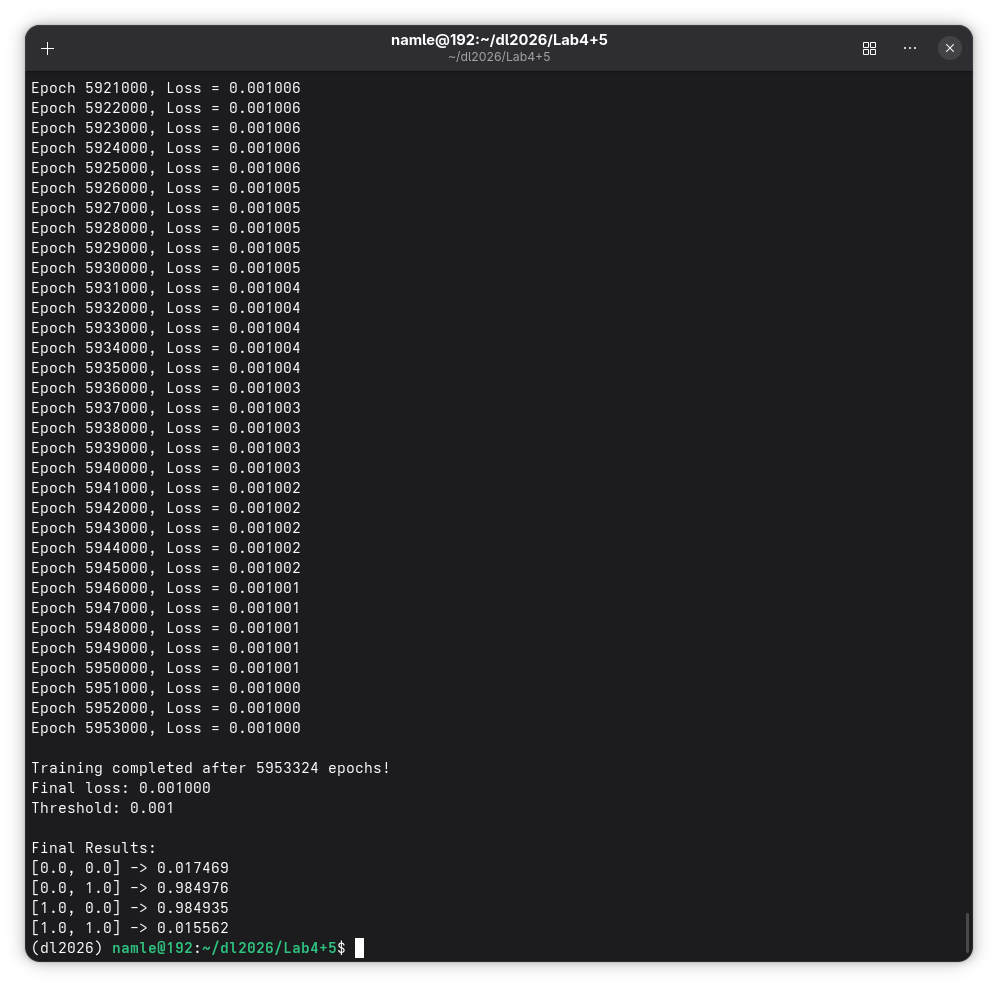
\includegraphics[width=0.9\linewidth]{backpro_results.png}
    \caption{Training process and final XOR results}
\end{figure}

\section{House Price Dataset}

The neural network was also tested with
the house price-size dataset from Labwork 2.

The network was able to reduce the loss
during training.

\end{document}